% Standalone editorial revision of the supplied final report, 20 October 2026.
% Experimental table values are preserved. Text, qualifications and repeated material were revised.
% Compile main.tex twice with the accompanying figures/ directory, or upload this folder to Overleaf.
% This is an edited snapshot; the original report generator does not maintain these revisions.
\documentclass[conference]{IEEEtran}
\IEEEoverridecommandlockouts
\usepackage[T1]{fontenc}
\usepackage{cite}
\usepackage{amsmath,amssymb,amsfonts}
\usepackage{graphicx}
\usepackage{textcomp}
\usepackage{xcolor}
\usepackage{array}
\usepackage{booktabs}
\usepackage{url}
\usepackage{tikz}
\usetikzlibrary{arrows.meta,positioning}

\definecolor{tumblue}{HTML}{0065BD}
\definecolor{tumdark}{HTML}{003359}
\newcolumntype{L}[1]{>{\raggedright\arraybackslash}p{#1}}
\newcommand{\tablenote}[1]{\par\smallskip{\footnotesize\raggedright #1\par}}

\begin{document}

\title{End-to-End Inventory Control via Monotonic Kolmogorov--Arnold Networks%
\thanks{Final report of an Interdisciplinary Project at the Chair of Logistics and Supply Chain Management, TUM
School of Management, Technical University of Munich, examined by Prof.~Dr.~Stefan Minner. Munich, October 2026.}}

\author{\IEEEauthorblockN{Qi Zhang}
\IEEEauthorblockA{\textit{Technical University of Munich}\\
Munich, Germany}
\and
\IEEEauthorblockN{Keming Lin}
\IEEEauthorblockA{\textit{Technical University of Munich}\\
Munich, Germany}
}

\maketitle

\begin{abstract}
Neural inventory policies can achieve high average profit while violating expected response directions. We study
monotonicity constraints in the lost-sales setting of Maggiar et al., comparing MonoKAN with an unconstrained KAN
under matched training protocols within each policy design. In the main design, the network predicts order quantity
from inventory, demand history and economics. The unconstrained KAN orders more as inventory rises on 8.7\%--51.3\%
of products across six runs; MonoKAN eliminates these reversals. The profit effect depends on the initialization
scheme: with constant initial outputs, MonoKAN earns 14.11 less per period (95\% CI for MonoKAN minus KAN:
$[-22.32,-5.90]$), whereas with open output layers it earns 548 more because the unconstrained KAN trains poorly.
These constraints guarantee response directions, not appropriate response magnitudes. In an alternative design, a
network chooses a demand percentile and a differentiable decoder produces an order-up-to target. Inventory
monotonicity then follows from the decoder, while MonoKAN constrains the economic mapping. The final alternative
policy reaches 0.80\% mean per-product regret; its mean-profit difference from KAN is not statistically significant.
Classical rules with the same demand information remain stronger on regret. The results show that the operational
effect of monotonic constraints depends on initialization and policy parameterization; they do not isolate a causal
relationship between the number of constrained inputs and profit.
\end{abstract}

\begin{IEEEkeywords}
Certified monotonicity, end-to-end learning, inventory control, Kolmogorov--Arnold networks, lost sales,
newsvendor problem
\end{IEEEkeywords}

% ================================================================ introduction
\section{Introduction}\label{sec:intro}
Every day a retailer decides how many units of each product to order. Too many, and the surplus ties up money and
shelf space; too few, and customers leave empty-handed. The classical approach estimates the demand distribution first
and then derives the order from it. End-to-end learning skips the separate forecast: a neural network observes the
state of the system, including the stock on hand, recent demand and the product's prices and costs, and outputs the
order directly, trained to maximise simulated profit. Maggiar et al.~\cite{maggiar2025} show that such a policy,
trained on synthetic products with known optimal benchmarks, comes within 0.41\% of the
omniscient benchmark in average profit.

Profit optimization alone does not ensure that the learned policy follows expected comparative statics. For example,
a policy may order more when inventory rises, holding demand history and economics fixed. Monotonic architectures
can enforce such directions for designated inputs~\cite{sill1998,you2017}.
MonoKAN~\cite{polomolina2024} is such an architecture: a Kolmogorov--Arnold network~\cite{liu2024} whose learned edge
functions are constrained to be monotone, which certifies the direction of every designated input for all possible
inputs.

We ask: \emph{how do monotonic constraints affect the behaviour and profit of an end-to-end inventory policy?}
We compare MonoKAN with an unconstrained KAN of the same architecture within each design. For direct quantity,
both models are tested under constant and open initialization schemes with the same calibration target
(Section~\ref{sec:main-design}); projection can still change their initial functions.

Following the examiner's feedback, the main design predicts the order quantity directly, so inventory monotonicity
must be enforced by the network. The alternative predicts a demand percentile and orders up to a learned target;
inventory monotonicity then follows from the decoder. This separates two uses of inventory knowledge, although the
comparison between designs changes several factors and is not an isolated ablation of the inventory constraint.

The project contributes:
\begin{itemize}
\item a direct-quantity MonoKAN policy that certifies the direction of all 37 inputs, and a matched comparison with
the same KAN without the certificate and with the feed-forward network of Maggiar et al.;
\item measurements of inventory reversals and profit differences under matched initialization schemes;
\item a soft-quantile target-stock policy with a monotone level network, the steps that took it from
21.4\% to 0.80\% regret, and comparisons with classical rules that use the
same information;
\item supporting analyses of economic responses, model size, decision time and the tested training-set sizes.
\end{itemize}

% ================================================================ setting
\section{Setting}\label{sec:setting}
\subsection{The Lost-Sales Inventory Problem}\label{sec:problem}
We use the synthetic lost-sales setting of Maggiar et al.~\cite{maggiar2025}. Each product has a selling price $p$, a
purchase cost $c$, a holding cost $h$ per unit left over at the end of a period and a penalty $k$ per unit of unmet
demand. Orders arrive immediately (no lead time) and unmet demand is lost. In period $t$ the policy sees the stock on
hand $I_t$ and orders $q_t \geq 0$; then demand $d_t$ is realised, and the period's profit and the next stock are
\begin{equation}
\begin{aligned}
r_t &= p\min(d_t,\, I_t + q_t) - c\,q_t \\
&\quad - h\,(I_t + q_t - d_t)^+ - k\,(d_t - I_t - q_t)^+,\\
I_{t+1} &= (I_t + q_t - d_t)^+.
\end{aligned}
\label{eq:dynamics}
\end{equation}
Demand is independent and identically distributed over time. Gamma samples, with product-specific mean $\mu$ and
coefficient of variation $\nu$, are rounded to nonnegative integers in the implementation. These parameters are hidden:
a learned policy observes economics and realized demand, initially 32 past observations. Demand is observed even when
sales are lost; this is not a censored-sales observation model. Products are drawn as in the
paper: $p$ exponential with mean 100, $c = p \cdot U$, $h$ exponential with mean 5, $k = 10 \cdot U$, $\mu$ exponential
with mean 100 and $\nu$ uniform on $(0, 1)$, with independent uniform draws $U$.

For the corresponding continuous-demand model, a base-stock policy orders up to the critical-fractile quantile of
the demand distribution~\cite{zipkin2000},
\begin{equation}
\begin{aligned}
S^* &= F^{-1}(\beta), \qquad \beta = \frac{p - c + k}{p - c + k + h},\\
q_t &= (S^* - I_t)^+.
\end{aligned}
\label{eq:newsvendor}
\end{equation}
This is the newsvendor solution. With the true Gamma parameters it defines the \emph{omniscient} benchmark: a
distribution-informed base-stock policy that knows the demand distribution but not the future demand. It is our
reference point, not a strict pathwise upper bound. It retains the continuous Gamma quantile rather than solving a
separate rounded-demand optimum; another policy can do better on a particular finite demand path.
Classical non-omniscient rules estimate $F^{-1}(\beta)$ from observed demand, either as an empirical quantile or by
fitting a Gamma distribution (Section~\ref{sec:protocol}).

\subsection{Training End to End Through the Simulator}\label{sec:training}
All learned policies are trained by DirectBackprop, as in the paper: the simulator in \eqref{eq:dynamics} is written
in a differentiable form, a policy runs a batch of products for a 100-period training horizon, and the gradient of the
profit objective flows through the simulated dynamics into the network's parameters. Each training product has a
fixed demand path; policies use only observations preceding the current action. Terminal stock receives a
purchase-cost credit, avoiding an artificial end-of-horizon write-off; holding costs still apply. Adam uses learning
rate 0.001. Each logged epoch is one optimizer update on a batch of 512 products sampled with replacement, rather
than a full pass through the catalogue. Runs use three training seeds (2025, 2026, 2027), with product-generation
seed fixed. Checkpoints maximize the validation version of the training objective: unweighted profit in the main
design and scaled profit in the final alternative.

\subsection{Measuring Performance}\label{sec:metrics}
Every policy is evaluated on the same 300 validation products and the same demand paths, over 520 periods of which
the first 20 are discarded to reduce initial-state effects. We report two measures.

\textit{Profit per period}, averaged over products, is the paper's measure. Product economics are heavy tailed
(profit per period has mean 4,284 and standard deviation 8,537 over
products), so this average is dominated by a few large products.

\textit{Regret} is the mean per-product shortfall against the omniscient policy, in percent:
\begin{equation}
\text{regret} = \frac{100}{|\mathcal{P}^+|} \sum_{i \in \mathcal{P}^+} \frac{R_i^* - R_i}{R_i^*},
\label{eq:regret}
\end{equation}
where $R_i$ and $R_i^*$ are the profits of the policy and the omniscient policy on product $i$. Every product counts
the same, so regret reveals failures on typical products that the average hides. The set $\mathcal{P}^+$ excludes the
21 of 300 products on which even the omniscient policy makes no profit, where a relative shortfall is meaningless.
The two measures can disagree: the initial direct-target model trailed a classical rule by 3.6\% in mean profit,
while its mean per-product relative shortfall was 21.4\%. This is an average relative loss, not a median-product result.

Because all policies face identical products and demand, we compare them \emph{paired by product}, which removes the
large product-to-product spread. For a difference in profit we first average each product's profit over the three
training seeds and then compare product by product. We report the mean difference with its 95\% confidence interval
and the paired t-test, the Wilcoxon signed-rank test, which is less sensitive to a few very large products, and the
share of products on which one policy is ahead. These tests treat the trained models as given: they describe variation
across products, not the variation from retraining with new seeds, which three seeds can only indicate.

% ================================================================ monokan
\section{Certified Monotonicity With MonoKAN}\label{sec:monokan}
\subsection{Kolmogorov--Arnold Networks}\label{sec:kan}
A multilayer perceptron applies fixed nonlinearities at its nodes and learns linear weights on its edges. A
Kolmogorov--Arnold network (KAN) does the reverse: every edge carries its own learnable univariate function, and nodes
only sum their incoming edges~\cite{liu2024}. A layer maps $x \in \mathbb{R}^n$ to
\begin{equation}
y_j = \sum_i \varphi_{ji}(x_i),\qquad \varphi_{ji}(x) = w^{b}_{ji}\, b(x) + w^{s}_{ji}\, s_{ji}(x),
\label{eq:kan}
\end{equation}
where $b$ is a fixed increasing base function (a shifted, positive ELU in our implementation) and $s_{ji}$ is a learned
cubic Hermite spline on a grid of knots, with the value and slope at each knot as parameters. Because each edge is a
curve of one variable, a trained KAN can be inspected edge by edge.

\subsection{Monotone Splines and the Certificate}\label{sec:certificate}
A sufficient condition for a cubic Hermite interval to be monotone is the Fritsch--Carlson
condition~\cite{fritsch1980}: for nonzero secant slope $\Delta$, the normalized endpoint slopes satisfy
$\alpha,\beta\geq0$ and $\alpha^2+\beta^2\leq9$. Flat intervals have zero endpoint slopes.
MonoKAN~\cite{polomolina2024} uses this to certify monotonicity. After every optimiser step we project the parameters
back onto the monotone set:
\begin{itemize}
\item for every input with a required direction, the first-layer edges get a base weight of that sign, a non-negative
spline weight, and a spline projected to be monotone in that direction (knot values made monotone, knot slopes given
the right sign and scaled until the Fritsch--Carlson condition holds);
\item every edge in later layers is projected to be increasing, with non-negative weights.
\end{itemize}
A sum of functions that move in one direction moves in that direction, and an increasing function of it keeps it. The
network's output is therefore monotone in every designated input, with the designated sign, for every possible input,
not only on the training data, up to floating-point rounding. Outside the knot range, linear extrapolation uses the
signed endpoint slopes. The guarantee concerns direction, not derivative magnitude or profit.

\subsection{Two Implementation Lessons}\label{sec:lessons}
Two defects in our first implementation are worth recording, because both changed results. First, the projection wrote
the conditions of neighbouring intervals one after the other, although adjacent intervals share a knot slope. The
second write could undo the first, leaving rare, tiny violations (worst case $5.6 \cdot 10^{-4}$). The corrected
projection combines both conditions at each knot, and a regression test checks it on uneven grids. Second, every
spline originally lived on a fixed grid from $-2$ to 4, while the normalised inputs did not. 63.8\% of demand
observations fell into the first of seven intervals, and holding cost and lost-sale penalty spanned less than one
interval. Those splines could barely bend, and the first model learned an almost constant policy. Placing the knots at
quantiles of the training data, the spline analogue of the grid update of Liu et al.~\cite{liu2024}, more than halved
the regret of our initial direct-target model (Section~\ref{sec:development}). After grid calibration, projection is
reapplied using the actual knot spacings to restore the monotonicity conditions.

% ================================================================ designs
\section{Two Policy Designs}\label{sec:designs}
Fig.~\ref{fig:designs} shows the two policy designs that we compare.

\begin{figure*}[!t]
\centering
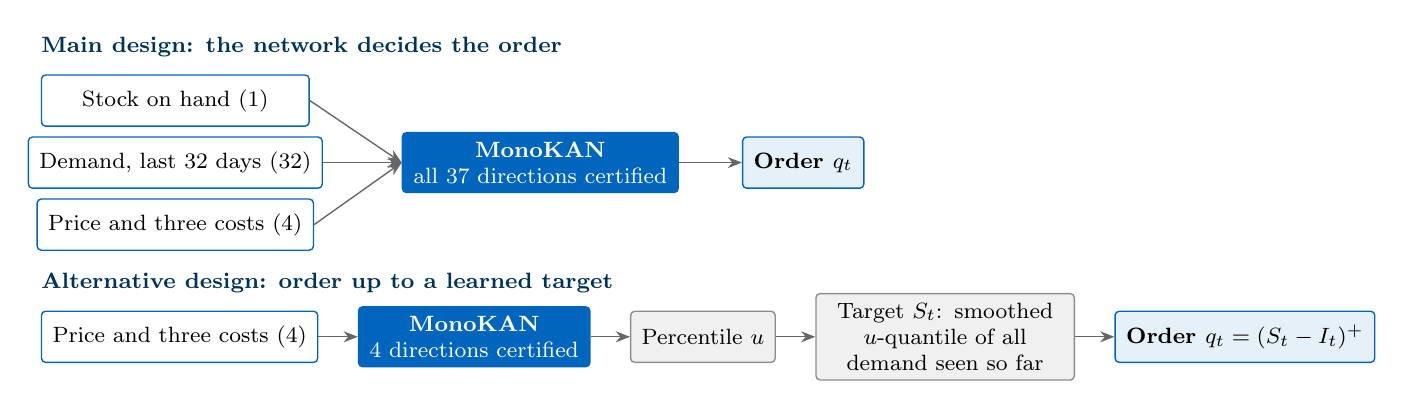
\begin{tikzpicture}[
  font=\footnotesize,
  box/.style={draw=tumblue, rounded corners=1.5pt, line width=0.5pt, minimum height=6.5mm, inner xsep=4pt,
              align=center},
  source/.style={box, minimum width=34mm},
  net/.style={box, fill=tumblue, text=white, font=\footnotesize\bfseries},
  fixed/.style={box, draw=black!45, fill=black!6},
  result/.style={box, fill=tumblue!10, font=\footnotesize\bfseries},
  flow/.style={-{Stealth[length=1.8mm, width=1.4mm]}, line width=0.5pt, black!60},
  heading/.style={font=\footnotesize\bfseries, text=tumdark, anchor=west, inner xsep=0pt}
]
\node[heading] at (0, 0) {Main design: the network decides the order};
\node[source, anchor=north west] (stock) at (0, -0.35) {Stock on hand (1)};
\node[source, below=1.2mm of stock] (demand) {Demand, last 32 days (32)};
\node[source, below=1.2mm of demand] (econ) {Price and three costs (4)};
\node[net, right=10mm of demand] (mono) {MonoKAN\\{\normalfont all 37 directions certified}};
\node[result, right=8mm of mono] (order) {Order $q_t$};
\foreach \source in {stock, demand, econ} \draw[flow] (\source.east) -- (mono.west);
\draw[flow] (mono) -- (order);
\node[heading] at (0, -3.0) {Alternative design: order up to a learned target};
\node[source, anchor=north west] (econ2) at (0, -3.35) {Price and three costs (4)};
\node[net, right=5mm of econ2] (mono2) {MonoKAN\\{\normalfont 4 directions certified}};
\node[fixed, right=5mm of mono2] (percentile) {Percentile $u$};
\node[fixed, right=5mm of percentile, text width=30mm] (target)
  {Target $S_t$: smoothed $u$-quantile of all demand seen so far};
\node[result, right=5mm of target] (order2) {Order $q_t = (S_t - I_t)^+$};
\draw[flow] (econ2) -- (mono2);
\draw[flow] (mono2) -- (percentile);
\draw[flow] (percentile) -- (target);
\draw[flow] (target) -- (order2);
\end{tikzpicture}
\caption{The two policy designs. In the main design the network decides the order, so the rule ``more stock, never a
larger order'' must come from the network. In the alternative it comes from the subtraction in the last step, and the
network only chooses a demand percentile from the economics. Blue: learned; grey: fixed computation.}
\label{fig:designs}
\end{figure*}

\subsection{Main Design: The Network Decides the Order}\label{sec:main-design}
The main design maps stock on hand, the last 32 demands and four economic quantities to the order:
$1 + 32 + 4 = 37$ inputs. With immediate arrivals there is no pipeline inventory. The required direction for each
input is fixed in advance (Table~\ref{tab:inputs}), and
MonoKAN certifies all 37. The demand inputs are sorted before entering the network. Each sorted value is
nondecreasing in every raw observation, so the certified directions carry over to the raw inputs. The output passes
through a softplus and is multiplied by the mean of the 32 observations available at the start, which makes the order
non-negative and proportional to the product's scale without changing any direction. In evaluation, but not in
training, the order is limited to $\max(4m_0-I_t,0)$, where $m_0$ is the initial historical mean floored at 1.
If stock already exceeds this threshold, the guard prevents further orders but cannot remove existing stock.
The guard preserves the specified directions and applies to all arms;
Section~\ref{sec:profit} reports its effect.

\begin{table}[!t]
\caption{Inputs of the Main Design and Their Certified Directions}
\label{tab:inputs}
\centering
\footnotesize
\setlength{\tabcolsep}{3pt}
\begin{tabular}{@{}L{25mm}rL{25mm}L{23mm}@{}}
\toprule
Input & Count & Certified rule & Reason \\
\midrule
Stock on hand & 1 & more stock $\rightarrow$ never order more & stock already covers demand \\
Demand in each of the last 32 periods & 32 & more demand $\rightarrow$ never order less & higher demand needs more
stock \\
Selling price & 1 & higher $\rightarrow$ never order less & a lost sale forgoes more margin \\
Lost-sale penalty & 1 & higher $\rightarrow$ never order less & running out costs more \\
Purchase cost & 1 & higher $\rightarrow$ never order more & each unit earns less margin \\
Holding cost & 1 & higher $\rightarrow$ never order more & leftover stock costs more \\
\bottomrule
\end{tabular}
\end{table}

MonoKAN uses one hidden layer of 8 nodes and Hermite splines with 5 intervals placed at data quantiles,
4,265 parameters in total. The comparison KAN has the same architecture and training but no
projection. Either network can start from one of two initialisations of its output layer. In the \emph{constant}
start the output-layer weights are zero, so every product starts at the same order per unit of mean demand: the
median empirical newsvendor level of the training products. In the \emph{open} start the weights are nonzero, so the
initial order already varies with the inputs, and the bias is shifted so that the median initial order on reference
contexts equals that level. Our first runs started MonoKAN open and the KAN constant. Because the start turned out to
matter, we tested both networks under each initialization scheme (Section~\ref{sec:profit}). Constant starts give
the same initial actions; open starts share the calibration target but need not give identical initial functions
after projection. The third arm is a causal-CNN/FCNN implementation following Maggiar et al. with
2,105 parameters and its own initialisation. All arms are trained on the same 1,000 products for
2,400 epochs to maximise total profit.

To check the stock rule we sweep the stock on hand of every validation product from 0 to 4 days of mean demand in 25
steps, holding all other inputs at the product's observed values, and flag every step at which the order rises (by
more than $10^{-4}$ of a day's demand). For each product, a linear fit over stock from 0 to 1.5 days of mean demand
measures the average response; coefficients are then averaged over products and seeds. This statistic is not a
pointwise derivative bound. An order-up-to policy has derivative $-1$ while ordering and 0 otherwise; the reference
policy's average fitted slope is $-$0.90.

\subsection{Alternative Design: Order Up to a Learned Target}\label{sec:alternative-design}
Equation~\eqref{eq:newsvendor} suggests a different structure: let the network choose only the percentile, and let a
fixed formula turn it into an order. A small MonoKAN level network reads only the four economic inputs and outputs a
percentile $u = \sigma(f(p, c, h, k))$. The target stock is a smoothed empirical quantile of all demand observed so
far. With $z_{(1)} \leq \dots \leq z_{(n)}$ the sorted observations and $t_j = (j - 1)/(n - 1)$ their positions,
\begin{equation}
\begin{aligned}
S_t &= g(u) \Bigl[ z_{(1)} + \sum_{j=2}^{n} \sigma\Bigl(\frac{u - t_j}{\tau_n}\Bigr) \bigl(z_{(j)} - z_{(j-1)}\bigr)
\Bigr],\\
q_t &= (S_t - I_t)^+,
\end{aligned}
\label{eq:soft-quantile}
\end{equation}
where the final configuration measures smoothing in order-statistic counts:
$\tau_n=\max(\operatorname{softplus}(\eta),10^{-4})/(n-1)$, for $n\geq2$, with learned $\eta$.
The positive gain $g(u)=\exp(a u+b)$ has learned bias $b$ and nonnegative slope
$a=\operatorname{softplus}(\rho)$. The weights $w_j = \sigma((u - t_j)/\tau_n)$ lie in $(0, 1)$ and decrease in $j$, because the positions $t_j$
increase. Rearranged, the bracket in \eqref{eq:soft-quantile} is
\[
(1 - w_2)\, z_{(1)} + \sum_{j=2}^{n-1} (w_j - w_{j+1})\, z_{(j)} + w_n z_{(n)},
\]
a combination of the order statistics with non-negative coefficients; each order statistic is nondecreasing in every observed demand, and the positive gain
preserves this, so $S_t$ is nondecreasing in every observed demand. $S_t$ increases with $u$, which MonoKAN makes
increase in price and penalty and decrease in purchase and holding cost. And the subtraction makes the order
nonincreasing in stock for \emph{any} level network. MonoKAN therefore constrains only the four economic inputs.
The level network has two layers of 8 nodes and 7-interval splines, with 1,889 parameters. The complete policy has
1,892, including temperature and the two gain parameters. It is trained on 5,000 products with a scaled objective: each
product's simulated profit is divided by $p_i \hat{\mu}_i T$, its price times its observed mean demand times the
horizon (each floored at 1), before averaging over products, so that a few large products do not dominate the
gradient.

The same decoder can use three kinds of demand information, which matters for fair comparisons: one fixed estimate
from the first 32 days, the last 32 days updated every period, or all demand seen so far (the final policy). Maggiar
et al.~\cite[Sec.~5.3.1]{maggiar2025} suggest such order-up-to structures, but warn that they are fragile: they only
work when the optimal policy is known to be of this form.

\subsection{Baselines and the Matched Protocol}\label{sec:protocol}
Besides the omniscient policy, we use two classical rules that estimate the target from observed demand: the
empirical quantile at the critical fractile, and a Gamma distribution fitted by the method of moments. The Gamma fit
explicitly assumes a Gamma demand family, whereas the learned policies acquire an implicit prior from Gamma-generated
training products. To match demand information, each rule is evaluated with each of the three windows:
\begin{itemize}
\item \textit{first 32 days, never updated}: how the paper defines its non-omniscient benchmarks;
\item \textit{last 32 days, updated daily}: what a policy in daily use sees, and the demand window of the main
design's inputs;
\item \textit{all demand seen so far}: the information of the final alternative policy.
\end{itemize}
Within each MonoKAN--KAN block, the models share products, demand paths, horizon, objective, update budget and
architecture. Initialization schemes are matched, except for the explicitly labeled first runs. Across policy designs,
other factors differ, including the decoder, architecture, initialization and evaluation guard. Checkpoints are
considered every 300 updates for the main design and every 150 for the matched alternative; the cross-design
comparison therefore does not isolate a single factor.

% ================================================================ results: main design
\section{Results: Main Design}\label{sec:results-main}
Table~\ref{tab:direct} reports the direct-quantity results for both initialization schemes and the reference policies.

\begin{table*}[!t]
\caption{Main Design Results}
\label{tab:direct}
\centering
\footnotesize
\begin{tabular}{@{}L{54mm}lrrrrr@{}}
\toprule
Policy & Start & Profit / period & Regret & Breaks & Reaction & Parameters \\
\midrule
MonoKAN (certified) & constant & 4,215.20 $\pm$ 5.64 & 14.60\% & 0.0\% & 0.46 & 4,265 \\
Same KAN, no certificate & constant & 4,229.31 $\pm$ 10.88 & 13.33\% & 35.1\% & 0.54 & 4,265 \\
MonoKAN (certified) & open & 4,206.43 $\pm$ 17.56 & 15.71\% & 0.0\% & 0.52 & 4,265 \\
Same KAN, no certificate & open & 3,658.28 $\pm$ 147.26 & 48.78\% & 23.6\% & 0.02 & 4,265 \\
Paper FCNN & --- & 3,874.38 $\pm$ 622.50 & 20.64\% & 0.0\% & 0.34 & 2,105 \\
Classical rules, last 32 days (empirical quantile / Gamma fit) & --- &
4,255.93 / 4,275.37 &
1.90\% / 1.25\% & 0.0\% & --- & --- \\
Omniscient base stock (knows the true distribution) & --- & 4,297.45 & 0.00\% & 0.0\% &
0.90 & --- \\
\bottomrule
\end{tabular}
\tablenote{Three seeds each, the same 300 validation products. ``Start'' is the output-layer initialisation
(Section~\ref{sec:main-design}). Profit per period $\pm$ standard deviation over seeds. ``Breaks'' is the share of
products on which the order rises with stock at some point of the sweep; ``reaction'' is the negative of the
product- and seed-averaged linear-fit coefficient, not a bound on local derivatives.}
\end{table*}

\subsection{Without the Certificate, the Stock Rule Breaks}\label{sec:breaks}
From the constant start, the KAN without the certificate orders more as stock rises on
35.1\% of products on average (Fig.~\ref{fig:violations}(a)). This happens in every training
run, but how often varies widely: 45.3\%, 8.7\% and 51.3\% of products for the three
seeds. The breaks occur at 3.7\% of all swept stock steps; most are small, but the
largest is an extra order of about 11\% of a day's demand. From the open start the KAN
breaks the rule on 19.7\%, 16.0\% and 35.0\% of products, but these breaks are tiny, at
most 0.2\% of a day's demand, because this KAN barely reacts to stock at all
(Section~\ref{sec:profit}). Fig.~\ref{fig:violations}(b) shows the largest reversal we found in any run; the break
rates above show how common reversals are. Over part of the stock range, the KAN's order goes \emph{up} as stock goes
up. The order of the certified MonoKAN on the same product never rises with stock. MonoKAN breaks the rule for no
start, seed or product, as its construction guarantees.

\begin{figure*}[!t]
\centering
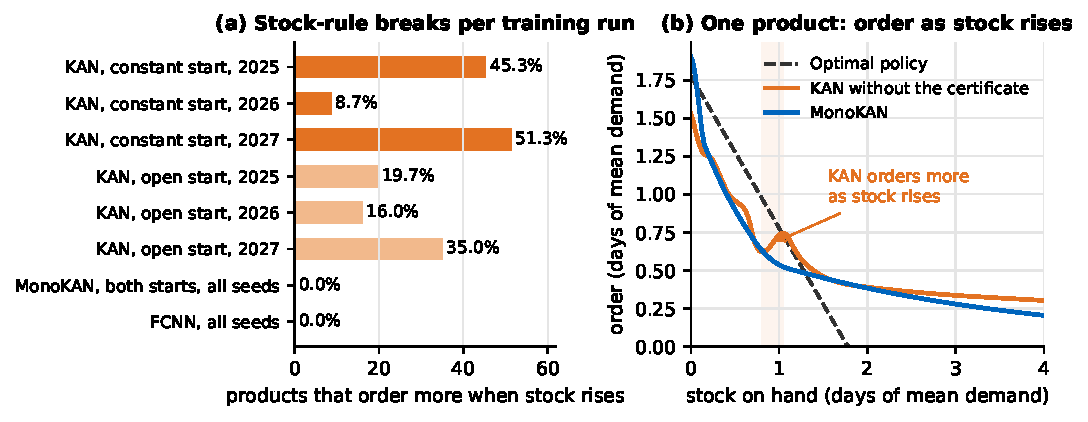
\includegraphics[width=\textwidth]{figures/fig_violations.pdf}
\caption{(a) Share of validation products on which the order rises with stock, for each training run of the KAN
without the certificate from the constant and the open start, and for MonoKAN (both starts) and the FCNN. (b) Order
against stock on hand for the product and run where the KAN breaks the rule most (constant start, seed 2027), with
MonoKAN from the open start and the same seed; both axes in days of mean demand. This worst-reversal illustration
is not a matched-initialization comparison. The reference policy orders up to its target one-for-one.}
\label{fig:violations}
\end{figure*}

The risk depends on the model family. The paper's FCNN did not break the rule in any of our three runs, while the KAN
did in all six runs. MonoKAN excludes this direction reversal by construction. Maggiar et al.~\cite[Sec.~5.3.3]{maggiar2025} instead add a soft penalty for violations
to the training loss, which makes breaks less likely but cannot exclude them.

\subsection{Profit With and Without the Certificate}\label{sec:profit}
Initialization changes the comparison (Table~\ref{tab:direct-paired}). With constant starts, MonoKAN earns 14.11
less per period, about 0.3\% of mean profit, and regret increases from 13.33\% to 14.60\%. This comparison concerns all
37 constraints together; it cannot separate the inventory constraint from the other directions, or representational
restriction from optimization difficulty. The table reports the product-level confidence intervals and tests.

From the open start the comparison reverses. The unconstrained KAN barely learns to react to stock: its order falls by
only 0.02 per unit of stock, against 0.54 from the constant start,
its regret is 48.78\%, and its profit varies widely between seeds. MonoKAN earns
548.15 more per period (95\% CI 390.33 to 705.97) and
is ahead on 82\% of products. MonoKAN itself depends far less on its start: it earns
8.78 less from the open start than from the constant one (95\% CI
0.50 to 17.06), the unconstrained KAN
571 less. We have not investigated why the open start fails for the unconstrained KAN. In these
runs the certificate thus did two things: it cost a little profit when both networks started well, and it kept
training reliable from a start at which the unconstrained network failed. Our first runs mixed the starts (MonoKAN
open, KAN constant) and showed a gap of 22.89; the part beyond the constant-start gap is
MonoKAN's own loss from its start.

\begin{table*}[!t]
\caption{MonoKAN Minus the Same KAN Without the Certificate, Main Design}
\label{tab:direct-paired}
\centering
\footnotesize
\begin{tabular*}{\textwidth}{@{\extracolsep{\fill}}L{60mm}rrrrr@{}}
\toprule
Start of the two networks & Difference & 95\% CI & t-test $p$ & Wilcoxon $p$ & MonoKAN ahead \\
\midrule
Both constant & $-$14.11 & [$-$22.32, $-$5.90] & 0.0008 & $<$ 0.0001 & 32\% \\
Both open & +548.15 & [+390.33, +705.97] & $<$ 0.0001 & $<$ 0.0001 & 82\% \\
MonoKAN open, KAN constant (first runs) & $-$22.89 & [$-$32.57, $-$13.20] & $<$ 0.0001 & $<$ 0.0001 & 28\% \\
\bottomrule
\end{tabular*}
\tablenote{Profit per period, paired over the 300 products with rewards averaged over seeds.}
\end{table*}

The evaluation cap of Section~\ref{sec:main-design} does not drive these results. Evaluated without it, MonoKAN trails
the KAN by 15.29 from the constant start (95\% CI 6.37 to
24.21) and leads by 749 from the open start. Without the cap every
network's regret is higher, by 0.8 to 1.6 points for the three that trained well and
far more for the open-start KAN, whose excessive orders the cap cuts.

The FCNN average includes a failed run: seed 2027 earns 3,155.76 (42.43\% regret), whereas the other two average
4,233.69. All three remain in the reported result. This shows substantial seed sensitivity in this setup, not a
general inferiority of FCNN policies.

\subsection{What the Certificate Cannot Fix}\label{sec:cannot-fix}
Monotonicity fixes response direction, not magnitude. The reference policy has an average fitted stock reaction of
0.90, compared with at most 0.54 among the direct-quantity networks (Fig.~\ref{fig:reaction}). These averages can
hide steep local declines and flat tails: the displayed MonoKAN curve, for example, has a local secant slope near
$-5.20$. Thus the networks do not already satisfy a pointwise slope bound of $[-1,0]$. The results show a mismatch
with the order-up-to response shape, but do not isolate its contribution to regret. This distinction between signs
and sensitivity magnitudes is also discussed by Maggiar et al.~\cite[Sec.~5.3.2]{maggiar2025}.

\begin{figure}[!t]
\centering
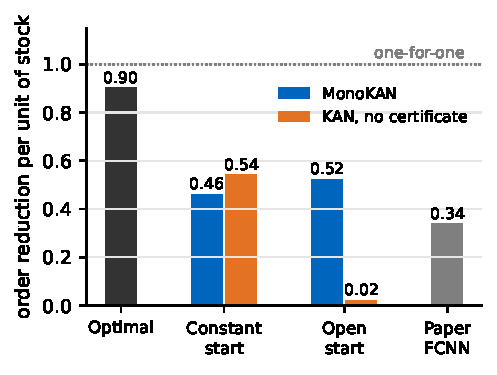
\includegraphics[width=\columnwidth]{figures/fig_reaction.pdf}
\caption{Negative linear-fit coefficient over stock from 0 to 1.5 days of mean demand, averaged over products and
seeds. This summarizes average response strength, not pointwise derivative bounds.}
\label{fig:reaction}
\end{figure}

No direct-quantity network comes close to a classical rule that uses the same 32-day window. The empirical quantile
and the Gamma fit on the last 32 days reach 1.90\% and
1.25\% regret, against 13.33\% or more for every network. The
paper's interpretability test points the same way. A direct-quantity policy's order at zero stock is its implied
order-up-to level. Per unit of mean demand, which removes product scale, MonoKAN's implied level correlates only
0.43 to 0.49 with the optimal level, depending on the start, and the
unconstrained KAN's 0.62 from the constant start, against 0.93 for the Gamma
fit on the same history. In raw units every policy looks good, because product scale alone explains most of the
variation. The certificate makes the direction of every input transparent, but the learned levels are only loosely
tied to the optimum.

% ================================================================ results: alternative design
\section{Results: Alternative Design}\label{sec:results-alt}
\subsection{From 21.4\% to 0.80\% Regret}\label{sec:development}
The first MonoKAN in this design, a deep network that output the target stock directly, reached
21.40\% regret, worse than an unconstrained FCNN in the same structure
(9.98\%) and about twelve times the regret of a classical rule. An unconstrained KAN of the
same architecture was similarly poor (20.68\%), so the constraint was not the main cause. Fig.~\ref{fig:development}
shows cumulative development changes, not independent one-factor ablations. All variants were designed to enforce monotonicity; the
projection defect of Section~\ref{sec:lessons} was corrected at the fourth step. The two largest gains came from
placing the spline knots where the data lies (Section~\ref{sec:lessons}) and from the soft-quantile structure
of~\eqref{eq:soft-quantile}. Using all demand seen so far, scaling each product's profit in the loss and training on
more products brought the regret to 0.80\%. On 3,000 validation products the final policy reaches
0.78\%.

\begin{figure*}[!t]
\centering
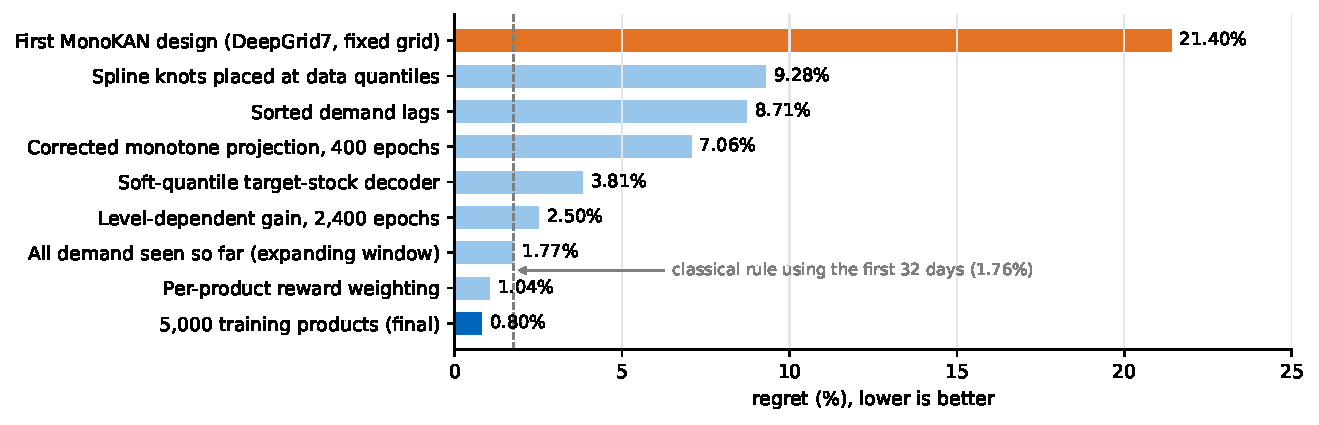
\includegraphics[width=\textwidth]{figures/fig_development.pdf}
\caption{Regret of the alternative design after each cumulative change, three seeds each. All variants were designed
to enforce monotonicity; the projection defect of Section~\ref{sec:lessons} was corrected at the fourth step.}
\label{fig:development}
\end{figure*}

Appendix~\ref{app:additional} retains negative results. A tested larger level network fitted the analytic fractile
less accurately; this alone does not establish lower control reward. Imitation warm-starting and a longer training
horizon did not improve the reported outcomes. A mismatch between static imitation targets and expanding-window
deployment may explain the warm-start result, but that cause was not isolated.

\subsection{Comparison at Matched Information}\label{sec:matched-information}
Table~\ref{tab:windows} and Fig.~\ref{fig:information} match the demand information available to each policy.
The expanding window gives the lowest regret for all four policies. Gamma fit performs best in every window;
the empirical quantile also outperforms the final alternative (0.27\% versus 0.80\%). Thus the alternative does
not improve on the strongest classical rules with matched information. Differences in window size must not be
credited to the neural architecture.

\begin{table}[!t]
\caption{Regret of Every Policy Within Each Kind of Information}
\label{tab:windows}
\centering
\footnotesize
\setlength{\tabcolsep}{3pt}
\begin{tabular}{@{}L{30mm}>{\raggedleft\arraybackslash}p{15mm}>{\raggedleft\arraybackslash}p{15mm}%
>{\raggedleft\arraybackslash}p{15mm}@{}}
\toprule
Policy & First 32 days, never updated & Last 32 days, updated daily & All demand seen so far \\
\midrule
Classical Gamma fit\textsuperscript{a} & 1.35\% & 1.25\% &
0.18\% \\
Classical empirical quantile & 1.76\% & 1.90\% &
0.27\% \\
Alternative design, KAN without certificate & 2.37\% & 1.96\% &
0.87\% \\
Alternative design, MonoKAN & 2.04\% & 1.83\% & 0.80\% \\
\bottomrule
\end{tabular}
\tablenote{Final setup (5,000 training products), three seeds, the same 300 validation products. The last two rows are
the same policy with and without the certificate. \textsuperscript{a}Also told that demand is Gamma distributed.}
\end{table}

\begin{figure*}[!t]
\centering
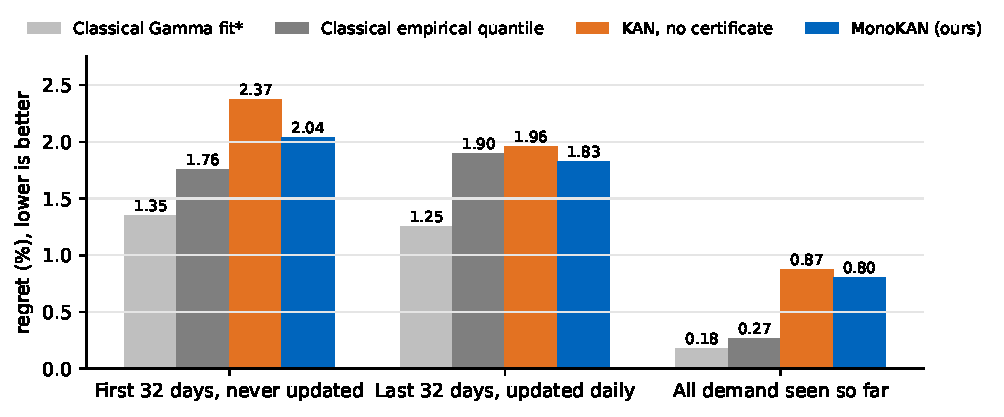
\includegraphics[width=\textwidth]{figures/fig_information.pdf}
\caption{The data of Table~\ref{tab:windows}. The first window is the paper's benchmark definition, the second is what
a policy in daily use sees, and the third is the final alternative policy's information.}
\label{fig:information}
\end{figure*}

\subsection{The Same KAN With and Without the Certificate}\label{sec:same-kan}
The last two rows of Table~\ref{tab:windows} are the core test of this design: the same policy, the same
1,892 parameters, the same training and data, once with and once without the certificate. MonoKAN has
the lower regret in all three windows. Table~\ref{tab:ts-paired} adds paired tests on profit. In the final setup with
all demand, the mean profit difference is $-$0.44 per period (95\% CI
$-$1.97 to +1.08, $p = 0.569$): we detected
no significant difference, which is not the same as showing that the profits are equal. MonoKAN is ahead on
61\% of products (Wilcoxon $p = 0.0001$). With the last 32 days the gain
is small but consistent; with the fixed estimate it is borderline, since only the t-test finds it. In a smaller setup
matched to the main design (1,000 products, profit objective, last 32 days) the certified model earned more:
+5.90 per period (95\% CI +3.32 to
+8.48), MonoKAN ahead on 72\% of products, and regret
2.26\% against 3.35\%.

\begin{table*}[!t]
\caption{MonoKAN Minus the Same KAN Without the Certificate, Alternative Design}
\label{tab:ts-paired}
\centering
\footnotesize
\setlength{\tabcolsep}{4pt}
\begin{tabular}{@{}L{38mm}rrrrrL{38mm}@{}}
\toprule
Setting & Difference & 95\% CI & t-test $p$ & Wilcoxon $p$ & MonoKAN ahead & Reading \\
\midrule
Final setup, all demand seen so far & $-$0.44 & [$-$1.97, +1.08] & 0.569 & 0.0001 & 61\% & no significant mean difference; ahead on most products \\
Final setup, last 32 days & +1.81 & [+0.16, +3.46] & 0.032 & $<$ 0.0001 & 62\% & small but consistent \\
Final setup, first 32 days & +2.64 & [+0.17, +5.10] & 0.036 & 0.464 & 51\% & small and borderline \\
1,000 products, profit objective, last 32 days & +5.90 & [+3.32, +8.48] & $<$ 0.0001 & $<$ 0.0001 & 72\% & ahead on both tests \\
\bottomrule
\end{tabular}
\tablenote{Profit per period, paired over the 300 products with rewards averaged over seeds.}
\end{table*}

The decoder supplies inventory monotonicity in both arms, so these comparisons concern the constrained economic
mapping. They do not explain why its profit effect changes with training setup. Earlier controls also show no
detected mean difference against a parameter-matched MLP ($-$0.08, $p=0.94$), and a gain of +6.73 over KAN with
a running-mean decoder ($p=0.0001$). Those blocks use different settings and should not be pooled with Table~\ref{tab:ts-paired}.

\subsection{Interpretability, Speed and Data Needs}\label{sec:interpretability}
With only four inputs the level network is easy to read (Fig.~\ref{fig:interpretability}(a)). The learned target
stock rises with price and penalty and falls with purchase and holding cost, as certified. The learned percentile $u$
also tracks the newsvendor fractile $\beta$ of \eqref{eq:newsvendor} closely, with correlation
0.982 (Fig.~\ref{fig:interpretability}(b)), although the fractile was never given to the model as
an input, an initial value or a training target. This shows agreement in the level, not that the policy equals the
textbook one: the quantile-based, order-up-to structure was supplied by design, and the decoder has its own learned
smoothing and gain.

\begin{figure*}[!t]
\centering
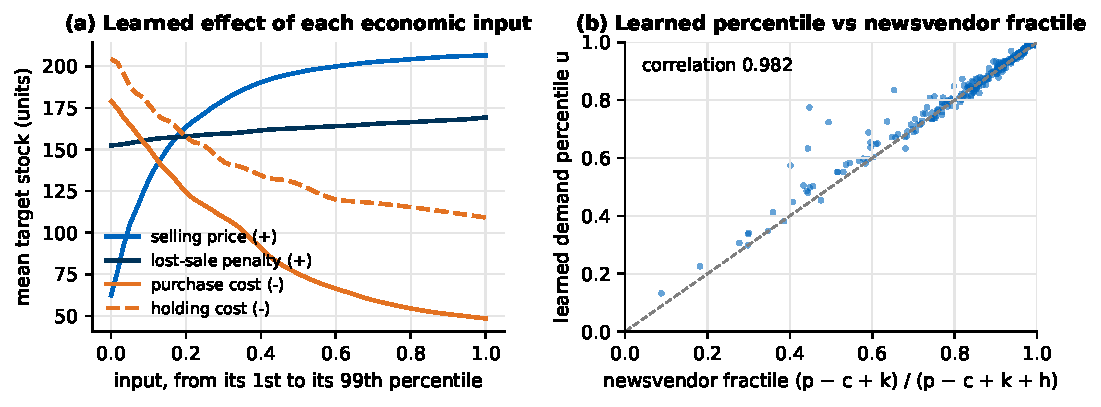
\includegraphics[width=\textwidth]{figures/fig_interpretability.pdf}
\caption{(a) Mean target stock as each economic input sweeps from its 1st to its 99th percentile, with the other
inputs at their observed values; the certified direction is in brackets. (b) Learned percentile against the analytic
newsvendor fractile for the 300 validation products. Both panels use the stored seed-2025 checkpoint; mean curves
illustrate its responses but are not, by themselves, a global certificate.}
\label{fig:interpretability}
\end{figure*}

The final policy has 1,892 parameters, against 15,297 for the earlier DeepGrid7 direct-target model. It is still slower per
decision than a feed-forward network of the same size (0.47~ms against
0.06~ms on a CPU), because spline evaluation is more expensive than a matrix product. These measured latencies are
small relative to a daily ordering interval. The experiment does not show a general data-efficiency advantage.
With 100 training products MonoKAN is worse
than a parameter-matched MLP (Fig.~\ref{fig:sample}). Across the three tested training-set sizes (three seeds each),
MonoKAN's regret fell steadily, while the MLP's rose again at 1,000 products; other sizes, budgets or initialisations
may behave differently.

\begin{figure}[!t]
\centering
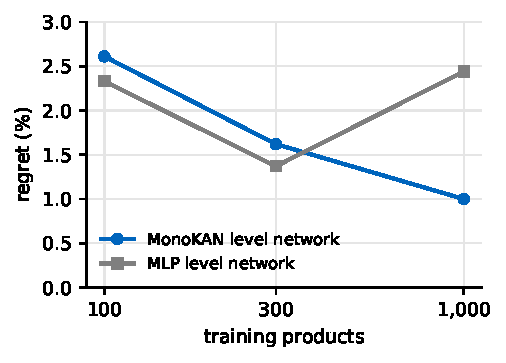
\includegraphics[width=\columnwidth]{figures/fig_sample_efficiency.pdf}
\caption{Regret of the alternative design against the number of training products, MonoKAN and a parameter-matched
MLP level network.}
\label{fig:sample}
\end{figure}

% ================================================================ comparison
\section{The Two Designs Side by Side}\label{sec:comparison}
Table~\ref{tab:designs} compares the designs at 1,000 training products, 2,400 updates, an unweighted profit objective
and three seeds, using the last 32 observations. The remaining protocol differences are described in
Section~\ref{sec:protocol}.

\begin{table}[!t]
\caption{Both Designs at Matched Training Size, Update Budget and Demand Window}
\label{tab:designs}
\centering
\footnotesize
\setlength{\tabcolsep}{3pt}
\begin{tabular}{@{}L{27mm}L{31mm}L{22mm}@{}}
\toprule
 & Main design: direct quantity & Alternative: target stock \\
\midrule
Who enforces ``more stock, never a larger order'' & the certificate & the subtraction $(S - I)^+$ \\
Without the certificate: products breaking the stock rule & 8.7--51.3\% per run & 0\%
(impossible) \\
Certified minus unconstrained KAN under the same initialization scheme, profit per period & $-$14.11
($p = 0.0008$) from the constant start; +548.15 from the open start &
+5.90 ($p < 0.0001$) \\
Regret of MonoKAN & 14.60\% (constant start), 15.71\%
(open) & 2.26\% \\
\bottomrule
\end{tabular}
\end{table}

The target-stock design has substantially lower regret in this comparison. Its decoder encodes a known structure,
but architecture, initialization, checkpoint frequency and the evaluation guard also differ. The result therefore
supports the combined policy design, not a causal claim that constraining more inputs necessarily costs more profit.
With an expanding window, the corresponding 1,000-product alternative reaches 1.62\% regret.

The direct-quantity formulation remains the main test of inventory monotonicity because it does not obtain that rule
from a decoder. The alternative exploits a known solution structure, which can be inappropriate in other settings.
For example, Maggiar et al.~\cite[Table~4]{maggiar2025} report DRL profit improvements of 0.79\%--5.68\% over their
standard base-stock benchmark with lead times of 2--7 periods. This is their baseline-relative profit improvement,
not the regret measure used here. Their warning about tailored structures~\cite[Sec.~5.3.1]{maggiar2025} motivates
testing broader settings; our experiments do not establish an advantage there.

% ================================================================ discussion
\section{Discussion}\label{sec:discussion}
\subsection{Why Impose Monotonicity if Profit Is the Objective?}\label{sec:why-monotone}
Restricting a fixed policy class cannot increase its maximum training objective. Finite-data training and
optimization, however, need not find the same solution with and without constraints. The open-start comparison
illustrates that a constraint can coincide with substantially better training outcomes; the constant-start
comparison shows a modest mean-profit cost. Neither establishes a universal effect.

We treat monotonicity as an explicit behavioural requirement. It excludes selected reversals beyond the finite
states checked after training, while profit and regret measure operational performance on the evaluation products.
These are different criteria. The current experiments support direction guarantees, not general claims of superior
profit, sample efficiency or robustness.


\subsection{Limitations}\label{sec:limitations}
\begin{itemize}
\item \textit{A simple setting.} Demand is stationary, orders arrive immediately and products are synthetic. This is
exactly the setting in which order-up-to is optimal, and it favours the alternative design. We have not tested
changing demand, lead times or real data.
\item \textit{Scale.} We train on 1,000 to 5,000 products, compared with 40,000 in the paper, and use three seeds per
experiment. Our absolute profit levels are therefore not comparable with the paper's.
\item \textit{Selection on the validation products.} Checkpoints are selected, and the method was developed, on the
same 300 validation products that we report on. Pairing on shared products and demand paths reduces product-level
noise, but it does not remove this selection bias. The final alternative policy keeps its standing on 3,000 products
(0.78\%), but that set contains the original 300 and is not a fully independent test
(Appendix~\ref{app:additional}).
\item \textit{Two starts, one evaluation cap.} The main design's comparison depends on the initialisation, and we
tested two starts; other starts, learning rates or budgets could move the cost of the certificate either way. Its
evaluation caps orders, which its training does not (Section~\ref{sec:main-design}); the cap applies to all arms alike
and does not change our conclusions (Section~\ref{sec:profit}).
\item \textit{Response shape is unexplained.} Average fitted stock reactions are weaker than the reference, but
local slopes can also be too steep. Limited training-state coverage is one possible explanation; it has not been
isolated experimentally.
\item \textit{Model family.} The stock-rule breaks are a property of the KAN family in our runs. The paper's FCNN did
not break the rule, so how often an unconstrained model breaks it depends on the model.
\item \textit{Training setup.} The main design has not been tested with the alternative's larger training set and
scaled objective. Whether these changes help direct-quantity policies remains unknown.
\end{itemize}

% The two page-wide appendix tables are defined here so that they come out at the top of the page on which
% the appendices start: LaTeX sets a page-wide float at the top of the page after the one it is defined on.
\begin{table*}[!t]
\caption{Commands That Reproduce the Results}
\label{tab:commands}
\centering
\footnotesize
\begin{tabular}{@{}L{48mm}>{\raggedright\arraybackslash\ttfamily}p{125mm}@{}}
\toprule
Result & \normalfont Command \\
\midrule
Main design, all five arms (Tables~\ref{tab:direct}, \ref{tab:direct-paired}, \ref{tab:designs};
Figs.~\ref{fig:violations}, \ref{fig:reaction}) &
python scripts/run\_direct\_quantity\_comparison.py train -{}-out outputs/direct\_quantity\newline
python scripts/run\_direct\_quantity\_comparison.py summarize outputs/direct\_quantity\newline
python scripts/run\_direct\_quantity\_comparison.py interpret outputs/direct\_quantity\newline
python scripts/run\_direct\_quantity\_comparison.py curves outputs/direct\_quantity\newline
python scripts/run\_direct\_quantity\_comparison.py cap outputs/direct\_quantity \\
Final alternative policy & python scripts/run\_soft\_quantile\_monokan.py -{}-seed 2025 -{}-output-dir
outputs/ts\_monokan/seed\_2025 \\
Same policy without the certificate & \ldots{} -{}-set monokan.level\_network=kan \\
Last 32 days only / first 32 days only & \ldots{} -{}-set monokan.window\_mode=sliding \quad / \quad \ldots{} -{}-set
monokan.roll\_history=false \\
Setup matched to the main design (Table~\ref{tab:designs}) & -{}-config
configs/paper\_lost\_sales\_soft\_quantile\_monokan\_profit.yaml -{}-set epochs=2400 -{}-set
idp\_benchmark.compact.reward\_epochs=2400 -{}-set idp\_benchmark.compact.validation\_interval=150 -{}-set
monokan.window\_mode=sliding \\
Classical rules in every window (Table~\ref{tab:windows}) & python scripts/run\_classical\_windows.py \\
Regret and paired tests (Tables~\ref{tab:windows}, \ref{tab:ts-paired}) & python
scripts/compare\_target\_stock\_runs.py summary outputs/ts\_monokan outputs/ts\_kan\newline python
scripts/compare\_target\_stock\_runs.py pair outputs/ts\_monokan outputs/ts\_kan \\
Interpretability (Fig.~\ref{fig:interpretability}) & python
scripts/run\_monokan\_interpretability.py \ldots{} \\
This edited report, with its accompanying \texttt{figures/} directory & pdflatex main.tex\newline pdflatex main.tex \\
\bottomrule
\end{tabular}
\end{table*}

\begin{table*}[!t]
\caption{Training and Evaluation Settings}
\label{tab:protocol}
\centering
\footnotesize
\begin{tabular}{@{}L{34mm}L{56mm}L{38mm}L{38mm}@{}}
\toprule
Setting & Main design & Alternative, final & Alternative, matched \\
\midrule
Configuration (\texttt{configs/\allowbreak paper\_\allowbreak lost\_\allowbreak sales\_*.yaml}) &
\texttt{rolling\_\allowbreak direct\_\allowbreak target\_\allowbreak dev\_\allowbreak 1k\_\allowbreak normalized} &
\texttt{soft\_\allowbreak quantile\_\allowbreak monokan} &
\texttt{soft\_\allowbreak quantile\_\allowbreak monokan\_\allowbreak profit} \\
Training products & 1,000 & 5,000 & 1,000 \\
Optimizer updates (logged as epochs) & 2,400 & 2,400 & 2,400 \\
Batch size & 512 & 512 & 512 \\
Checkpoint interval (updates) & 300 & 150 & 150 \\
Objective & total profit & mean scaled profit, $R_i/(p_i\hat\mu_iT)$ & total profit \\
Demand information & last 32 days (order scaled by the initial 32-day mean) & all demand seen so far & last 32 days \\
Network & KAN 37--8--1, 5 intervals & \multicolumn{2}{L{78mm}@{}}{level network 4--8--8--1, 7 intervals} \\
Output initialisation & constant or open, both reported (Section~\ref{sec:main-design}) &
\multicolumn{2}{L{78mm}@{}}{same level-calibration scheme for MonoKAN and KAN} \\
Spline knots & \multicolumn{3}{L{138mm}@{}}{placed at quantiles of the training inputs} \\
Optimiser & \multicolumn{3}{L{138mm}@{}}{Adam, learning rate 0.001, best validation checkpoint} \\
Training horizon & \multicolumn{3}{L{138mm}@{}}{100 periods, fixed demand paths, terminal stock credited at purchase
cost} \\
Evaluation & \multicolumn{3}{L{138mm}@{}}{300 validation products, 520 periods, first 20 discarded, identical demand
paths for all policies} \\
Order cap & in evaluation only: stock after ordering at most 4$\times$ the initial 32-day mean &
\multicolumn{2}{L{78mm}@{}}{none} \\
Seeds & \multicolumn{3}{L{138mm}@{}}{2025, 2026, 2027} \\
\bottomrule
\end{tabular}
\end{table*}

% ================================================================ conclusion
\section{Conclusion}\label{sec:conclusion}
The experiments distinguish a monotone direct-order network from a policy whose decoder already encodes the
inventory response. In the direct design, MonoKAN prevents wrong-direction responses, but the reward comparison
with unconstrained KAN depends strongly on initialisation. The guarantee controls direction, not reaction magnitude:
the reported average fitted slopes do not establish a pointwise slope bound. In the structured alternative,
inventory monotonicity comes from the order-up-to decoder, while MonoKAN constrains the economic mapping. This
alternative reached 0.80\% regret, with no detected mean profit difference from its matched unconstrained KAN.
Classical rules using the same expanding information remained stronger in this setting. Differences between the
two designs cannot be attributed solely to the number of constrained inputs.

Further experiments should isolate the inventory constraint while keeping the other constraints and training
protocol fixed, and evaluate whether wider inventory-state coverage or explicit slope restrictions improve policy
behaviour. A bound between $-1$ and 0 would limit steep responses but would not itself force a stronger response to
stock. These questions, and evaluation on an independent protected population, remain open; changing demand or lead
times would require a separate study of whether the imposed policy structure remains appropriate.

% ================================================================ appendices
\appendices
\section{Reproducing the Results}\label{app:reproduce}
Commands in Table~\ref{tab:commands} run from the repository root. Install the project with
\texttt{python -m pip install -e ".[dev]"} and run tests with \texttt{python -m pytest -q}.
Target-stock training commands run one seed at a time and are repeated for seeds 2025, 2026 and 2027.
Training is not required to inspect the saved results. The twelve direct-design KAN summaries are in
\texttt{report/\allowbreak data/\allowbreak direct\_\allowbreak quantity}; their checkpoints are in
\texttt{outputs/\allowbreak direct\_\allowbreak quantity\_\allowbreak matched\_\allowbreak init}.
The three final alternative-policy runs are in \texttt{outputs/\allowbreak soft\_\allowbreak quantile\_\allowbreak monokan}
and can be summarised with \texttt{python scripts/\allowbreak compare\_\allowbreak target\_\allowbreak stock\_\allowbreak runs.py
summary outputs/\allowbreak soft\_\allowbreak quantile\_\allowbreak monokan}.
The submitted archive does not include the original report generator. This edited report is a standalone
\texttt{main.tex} with six accompanying figure PDFs. Some earlier FCNN and information-window per-run outputs
were not retained; their tabulated results therefore cannot all be rechecked from the submitted archive alone.

The generic saved target-stock diagnostic for the final soft-quantile wrapper includes an extra historical-mean
factor and should not be interpreted as its target level. Its empty spline-certification CSV is also not evidence of
certification. The structural argument instead requires the signed network paths, spline constraints and monotone
decoder described in Section~\ref{sec:monokan}; empirical plots alone do not establish a global guarantee.

\section{Protocol Details}\label{app:protocol}
Table~\ref{tab:protocol} lists the training and evaluation settings of both designs.

\section{Additional Results}\label{app:additional}
Table~\ref{tab:confirmation} evaluates the final alternative policy on a 3,000-product superset,
Table~\ref{tab:sample} gives its profit and regret by the number of training products, and Table~\ref{tab:negative}
lists the changes that did not improve it.

\begin{table}[!htbp]
\caption{Additional Evaluation on 3,000 Validation Products}
\label{tab:confirmation}
\centering
\footnotesize
\begin{tabular}{@{}L{45mm}rr@{}}
\toprule
Policy & Profit / period & Regret \\
\midrule
Omniscient base stock & 4,693.34 & 0.00\% \\
Soft-quantile MonoKAN, 5,000 products & 4,679.59 & 0.78\% \\
Soft-quantile MonoKAN, 1,000 products & 4,678.87 & 1.28\% \\
Classical Gamma fit, first 32 days & 4,671.74 & 1.46\% \\
Classical empirical quantile, first 32 days & 4,651.87 & 2.34\% \\
\bottomrule
\end{tabular}
\tablenote{The 3,000 products are a superset of the 300 used for checkpoint selection. The absolute profit level
differs from the main tables because the product draw differs; the ordering of policies is unchanged.}
\end{table}

\begin{table}[!htbp]
\caption{Alternative Design: Profit and Regret by Number of Training Products}
\label{tab:sample}
\centering
\footnotesize
\setlength{\tabcolsep}{4pt}
\begin{tabular}{@{}rrrrr@{}}
\toprule
 & \multicolumn{2}{c}{MonoKAN level network} & \multicolumn{2}{c}{MLP level network} \\
\cmidrule(lr){2-3}\cmidrule(l){4-5}
Products & Profit / period & Regret & Profit / period & Regret \\
\midrule
100 & 4,279.35 & 2.61\% & 4,285.05 & 2.33\% \\
300 & 4,282.60 & 1.62\% & 4,284.38 & 1.37\% \\
1,000 & 4,284.08 & 1.00\% & 4,278.53 & 2.44\% \\
\bottomrule
\end{tabular}
\tablenote{Three seeds, 2,400 epochs each.}
\end{table}

\begin{table}[!htbp]
\caption{Changes That Did Not Improve the Alternative Design}
\label{tab:negative}
\centering
\footnotesize
\setlength{\tabcolsep}{3pt}
\begin{tabular}{@{}L{28mm}L{55mm}@{}}
\toprule
Change & Outcome \\
\midrule
Imitation warm start from the classical rule & 8.61\% regret after 200 epochs. Static imitation and expanding-window
deployment differ; whether that mismatch causes the degradation was not isolated. \\
Larger level network ($3 \times 16$, 12 intervals) & Worse fit of the newsvendor fractile (RMSE 0.033 against 0.026
for $2 \times 8$). \\
Training horizon 250 instead of 100 & No gain (2.06\% regret). \\
Running mean on top of the expanding window & Worse by 6.8 profit per period; additional smoothing is a possible explanation. \\
Per-product normalisation of prices & Rejected: it breaks the certificate, because raising the price moves the cost
ratios in conflicting directions. \\
\bottomrule
\end{tabular}
\end{table}

% ================================================================ references
\begin{thebibliography}{00}
\bibitem{maggiar2025} A. Maggiar \textit{et al.}, ``Structure-informed deep reinforcement learning for inventory
management,'' 2025, arXiv:2507.22040. [Online]. Available: \url{https://arxiv.org/abs/2507.22040}
\bibitem{sill1998} J. Sill, ``Monotonic networks,'' in \textit{Advances in Neural Information Processing Systems 10}.
Cambridge, MA, USA: MIT Press, 1998, pp. 661--667.
\bibitem{you2017} S. You, D. Ding, K. Canini, J. Pfeifer, and M. Gupta, ``Deep lattice networks and partial monotonic
functions,'' in \textit{Advances in Neural Information Processing Systems 30}, 2017.
\bibitem{polomolina2024} A. Polo-Molina, D. Alfaya, and J. Portela, ``MonoKAN: Certified monotonic Kolmogorov--Arnold
network,'' \textit{Neural Networks}, vol. 196, Art. no. 108278, 2026, doi: 10.1016/j.neunet.2025.108278.
\bibitem{liu2024} Z. Liu \textit{et al.}, ``KAN: Kolmogorov--Arnold networks,'' 2024, arXiv:2404.19756. [Online].
Available: \url{https://arxiv.org/abs/2404.19756}
\bibitem{zipkin2000} P. H. Zipkin, \textit{Foundations of Inventory Management}. McGraw-Hill, 2000.
\bibitem{fritsch1980} F. N. Fritsch and R. E. Carlson, ``Monotone piecewise cubic interpolation,'' \textit{SIAM J.
Numer. Anal.}, vol. 17, no. 2, pp. 238--246, 1980.
\end{thebibliography}

\end{document}
